\documentclass[a4paper,11pt]{article}

% Kódování a jazyk
\usepackage[utf8]{inputenc}
\usepackage[T1]{fontenc}
\usepackage[czech]{babel}
\usepackage{lmodern}

% Matematika
\usepackage{amsmath,amssymb,amsfonts}

% Grafika a layout
\usepackage{graphicx}
\usepackage[margin=2.2cm]{geometry}
\usepackage{float}
\usepackage{booktabs}
\usepackage{array}
\usepackage{multirow}
\usepackage{caption}
\usepackage{subcaption}
\usepackage{enumitem}
\usepackage{fancyhdr}
\usepackage{xcolor}
\usepackage{hyperref}

\hypersetup{
    colorlinks=true,
    linkcolor=blue!60!black,
    citecolor=blue!60!black,
    urlcolor=blue!60!black
}

\graphicspath{{1E/}}

\pagestyle{fancy}
\fancyhf{}
\fancyhead[L]{\small Spolehlivost konstrukcí -- Úloha 1E}
\fancyhead[R]{\small Akademický rok 2025/2026}
\fancyfoot[C]{\thepage}
\renewcommand{\headrulewidth}{0.4pt}

\newcommand{\unit}[1]{\,\mathrm{#1}}
\newcommand{\E}[1]{\times 10^{#1}}

\captionsetup{font=small}

\begin{document}

\section{Příklad 1E -- Stochastické vyhodnocení vnitřních účinků nosníku}

\vspace{-2mm}

\subsection*{Zadání a výpočtový postup}

Úkolem bylo vykreslit průběhy vnitřních účinků po délce nosníku, tedy normálové síly \(N(x)\), posouvající síly \(T(x)\) a ohybového momentu \(M(x)\). Vnější zatížení bylo uvažováno jako stochastické. Náhodné veličiny byly popsány normálním a lognormálním rozdělením se středními hodnotami podle obr. \ref{fig:zadani} a variačním koeficientem \(v=0{,}1\).

Řešený nosník je znázorněn na obr. \ref{fig:zadani}. Na nosník působí koncentrovaný moment \(M_0\), síla \(F\) a rovnoměrné spojité zatížení \(q\) na převislém úseku.

\begin{figure}[H]
	\centering
	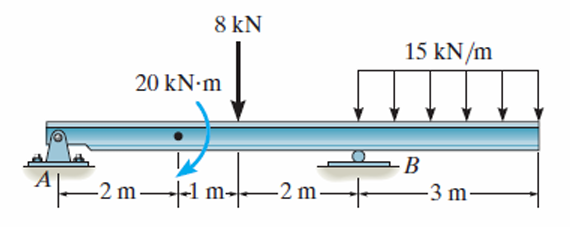
\includegraphics[width=0.92\textwidth,height=0.32\textheight,keepaspectratio]{zadani.png}
	\caption{Schéma zadání.}
	\label{fig:zadani}
\end{figure}

Pro výpočet reakcí bylo spojité zatížení nahrazeno výslednicí

\begin{equation}
	F_q = ql = 15 \cdot 3 = 45\,\mathrm{kN},
\end{equation}

která působí uprostřed zatíženého úseku, tedy v poloze \(x_q = 6{,}5\,\mathrm{m}\). Ze statických rovnic rovnováhy byly určeny reakce ve vazbách

\begin{equation}
	R_B = \frac{3F+19{,}5q+M_0}{5},
	\qquad
	R_A = F+3q-R_B.
\end{equation}

Pro střední hodnoty zatížení vychází

\begin{equation}
	R_A=-14{,}3\,\mathrm{kN}, \qquad
	R_B=67{,}3\,\mathrm{kN}, \qquad
	\max |M| = 67{,}5\,\mathrm{kN\,m}.
\end{equation}

\subsection*{Stochastické vyhodnocení}

Zatížení \(F\), \(q\) a \(M_0\) byla dále uvažována jako náhodné veličiny. Směrodatná odchylka jednotlivých veličin byla určena pomocí variačního koeficientu

\begin{equation}
	\sigma_X = v\mu_X,
	\qquad
	v=0{,}1.
\end{equation}

Výpočet byl proveden metodou Monte Carlo pro \(n = 1\,000\,000\) simulací. V každé simulaci byly vygenerovány náhodné hodnoty zatížení, ze kterých byly vypočteny reakce a průběhy vnitřních účinků. Byly porovnány dvě varianty rozdělení: normální a lognormální. Normální rozdělení je symetrické kolem střední hodnoty, zatímco lognormální rozdělení připouští pouze kladné hodnoty.

\begin{figure}[H]
	\centering
	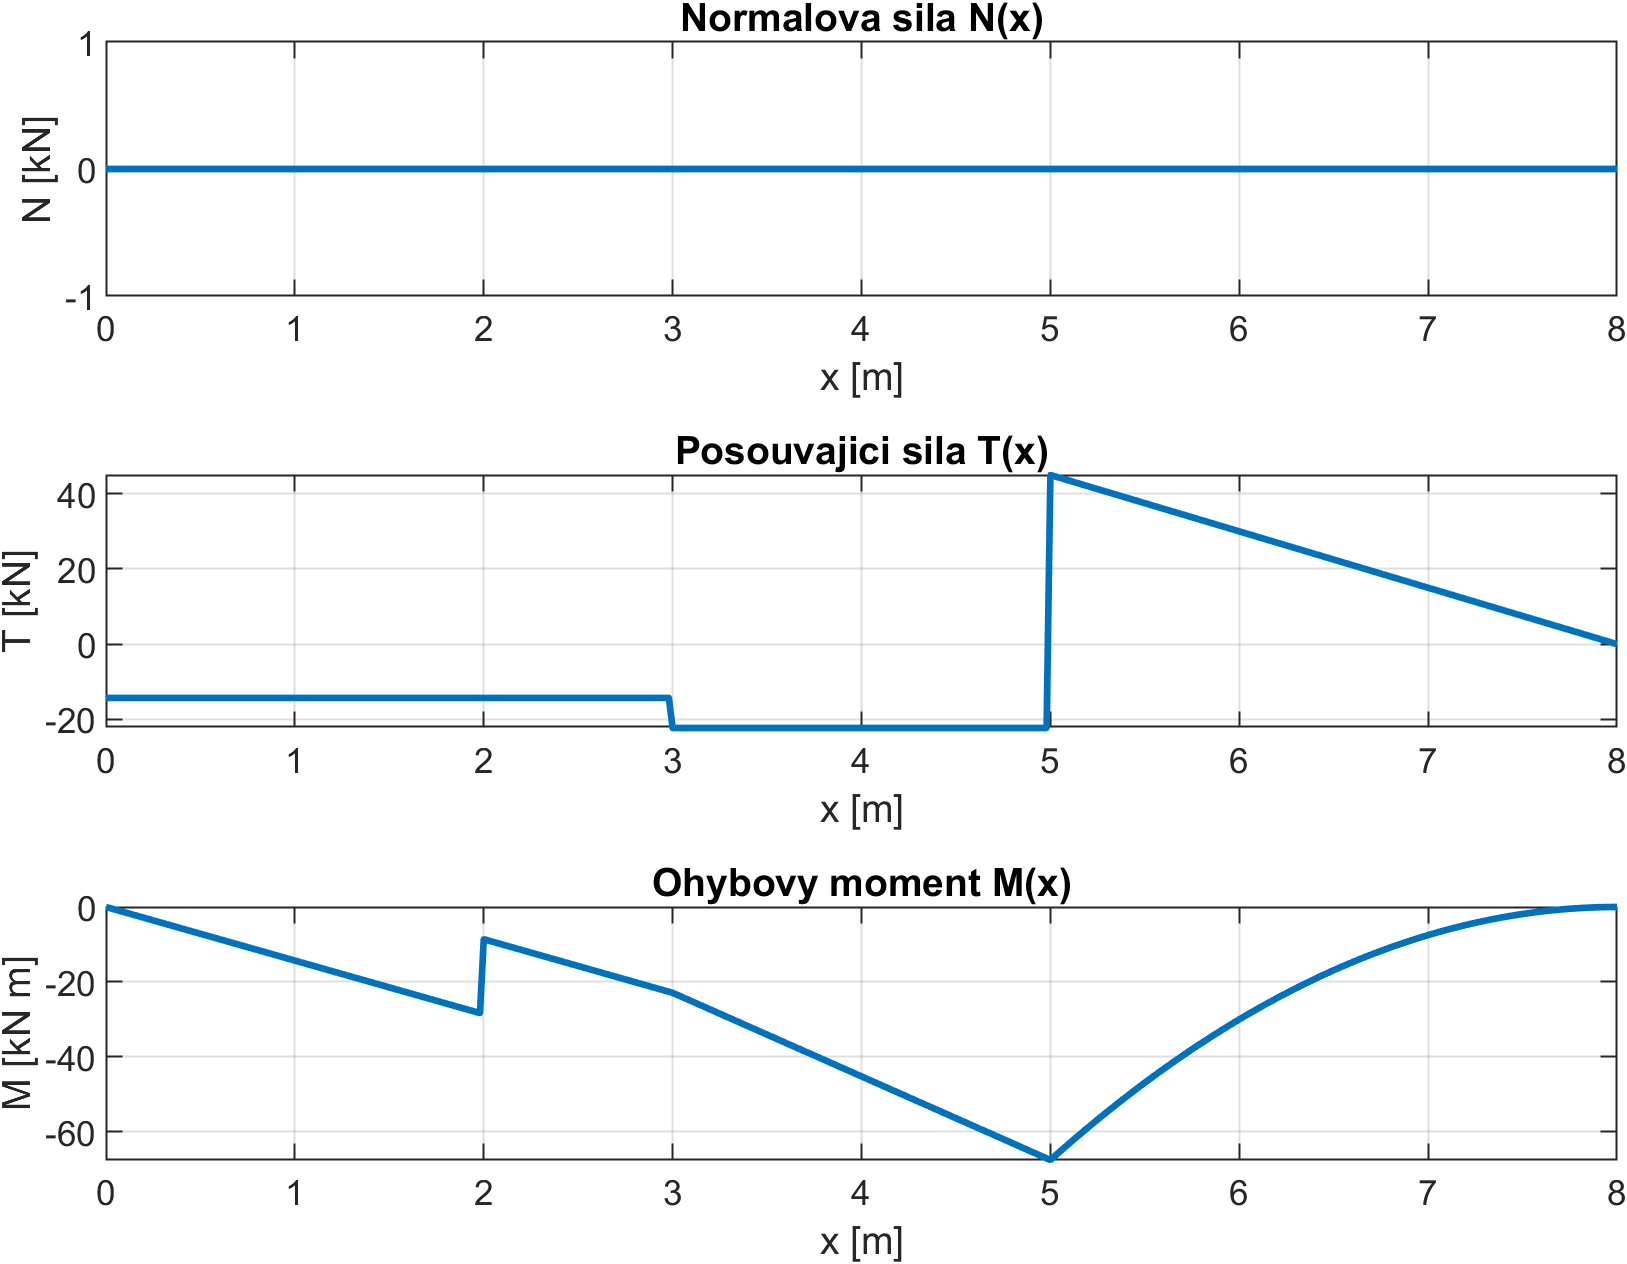
\includegraphics[width=0.82\textwidth,height=0.30\textheight,keepaspectratio]{01_deterministicke_prubehy.png}
	\caption{Deterministické průběhy \(N(x)\), \(T(x)\) a \(M(x)\) pro střední hodnoty zatížení.}
	\label{fig:det}
\end{figure}

\subsection*{Výsledky}

Na obr. \ref{fig:det} jsou uvedeny deterministické průběhy vnitřních účinků. Normálová síla je po celé délce nosníku nulová, protože na nosník nepůsobí vodorovné zatížení. Posouvající síla \(T(x)\) má skoky v místech bodových účinků a na převislé části lineárně klesá vlivem spojitého zatížení. Ohybový moment \(M(x)\) má v místě koncentrovaného momentu skok a na převislé části parabolický průběh.

\begin{table}[H]
	\centering
	\caption{Statistické výsledky pro \(1\,000\,000\) simulací.}
	\label{tab:vysledky}
	\scriptsize
	\begin{tabular}{llrrrr}
		\toprule
		\textbf{Rozdělení} & \textbf{Veličina} & \textbf{Průměr} & \textbf{Směr. odch.} & \textbf{P05} & \textbf{P95} \\
		\midrule
		Normální
		& \(R_A\,[\mathrm{kN}]\) & \(-14{,}298\) & \(1{,}4451\) & \(-16{,}673\) & \(-11{,}922\) \\
		& \(R_B\,[\mathrm{kN}]\) & \(67{,}294\) & \(5{,}8869\) & \(57{,}613\) & \(76{,}978\) \\
		& \(\max |M|\,[\mathrm{kN\,m}]\) & \(67{,}492\) & \(6{,}7547\) & \(56{,}388\) & \(78{,}604\) \\
		\midrule
		Lognormální
		& \(R_A\,[\mathrm{kN}]\) & \(-14{,}302\) & \(1{,}4452\) & \(-16{,}774\) & \(-12{,}027\) \\
		& \(R_B\,[\mathrm{kN}]\) & \(67{,}307\) & \(5{,}8852\) & \(58{,}136\) & \(77{,}446\) \\
		& \(\max |M|\,[\mathrm{kN\,m}]\) & \(67{,}507\) & \(6{,}7530\) & \(56{,}989\) & \(79{,}151\) \\
		\bottomrule
	\end{tabular}
\end{table}

Hodnoty P05 a P95 představují 5\% a 95\% percentil. Mezi těmito mezemi se nachází přibližně 90~\% simulovaných výsledků. Tyto hodnoty proto vyjadřují interval, ve kterém se nachází většina výsledků, a současně popisují jejich rozptyl způsobený náhodností zatížení.

\begin{figure}[H]
	\centering
	
	\begin{minipage}[t]{0.49\textwidth}
		\centering
		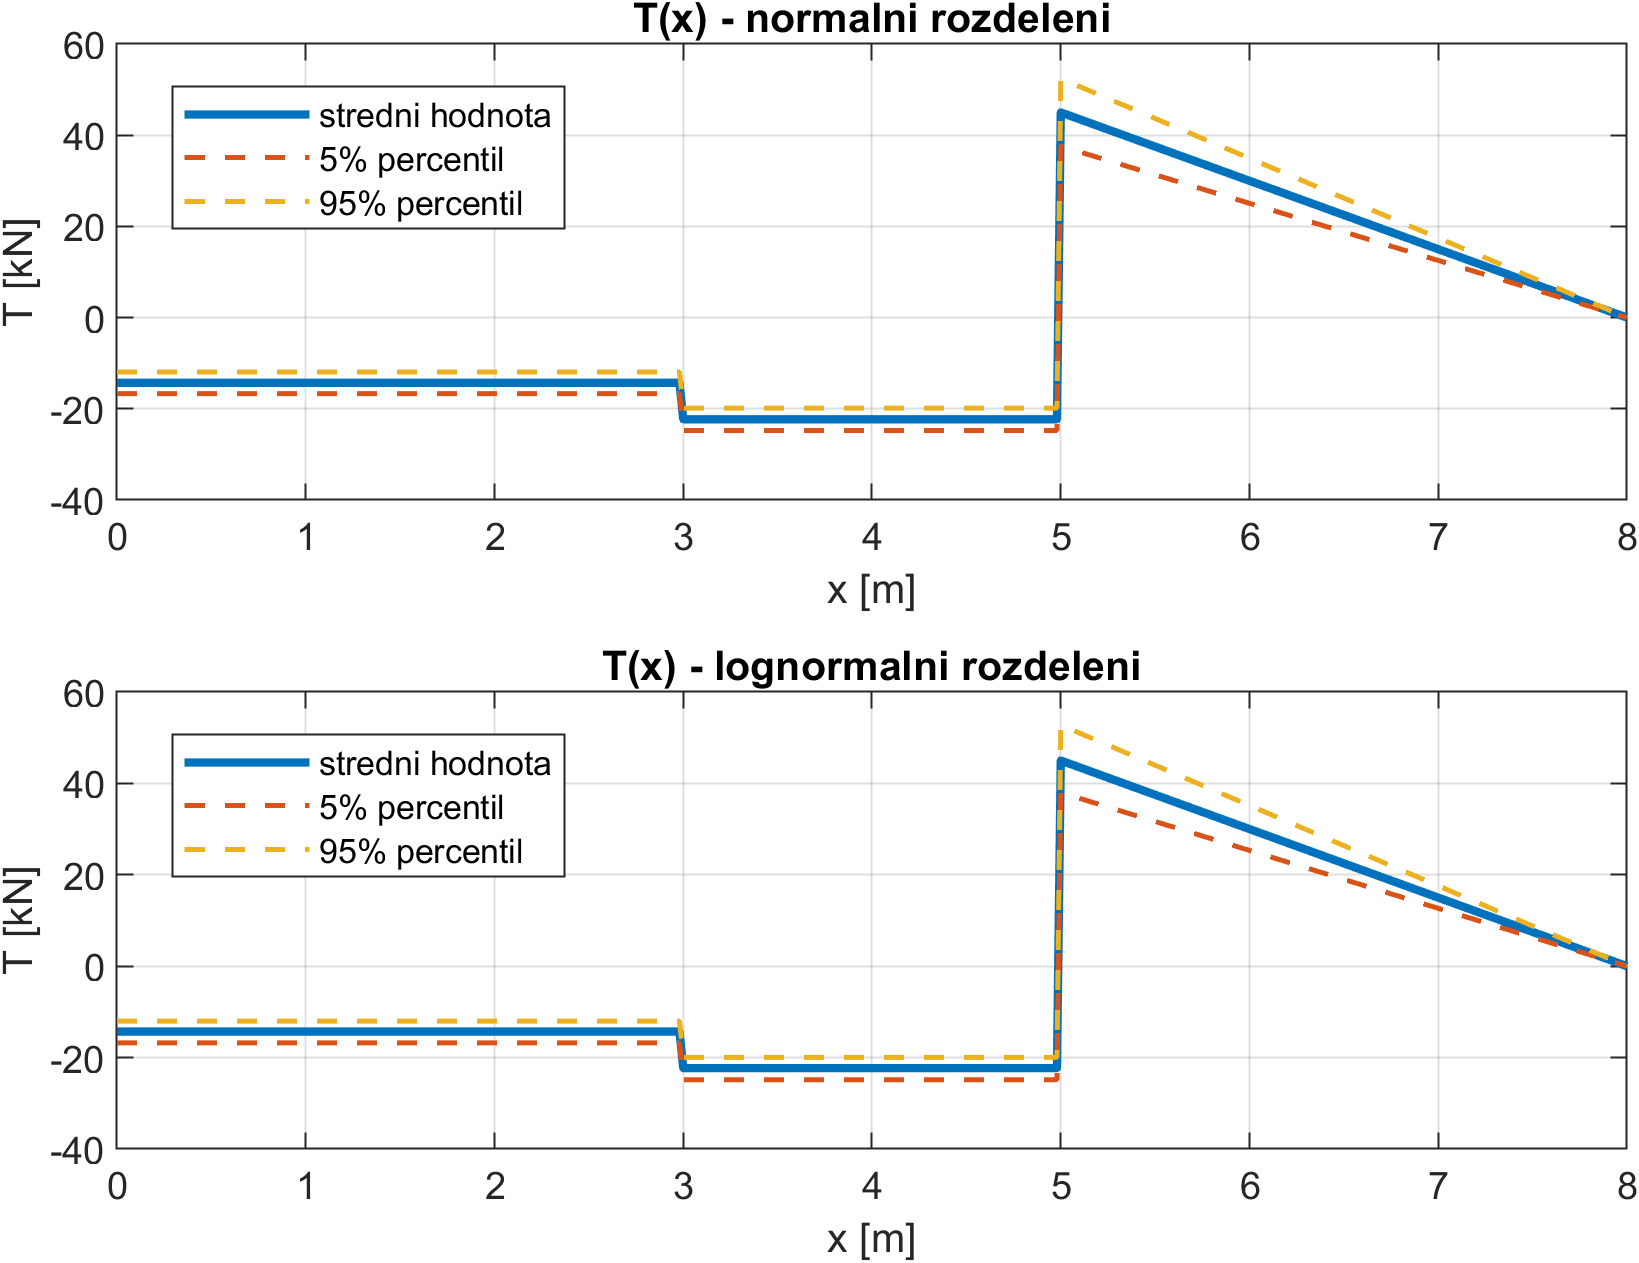
\includegraphics[width=\textwidth,height=0.30\textheight,keepaspectratio]{02_stochasticky_prubeh_T.png}
		{\small (a) Posouvající síla \(T(x)\)}
	\end{minipage}
	\hfill
	\begin{minipage}[t]{0.49\textwidth}
		\centering
		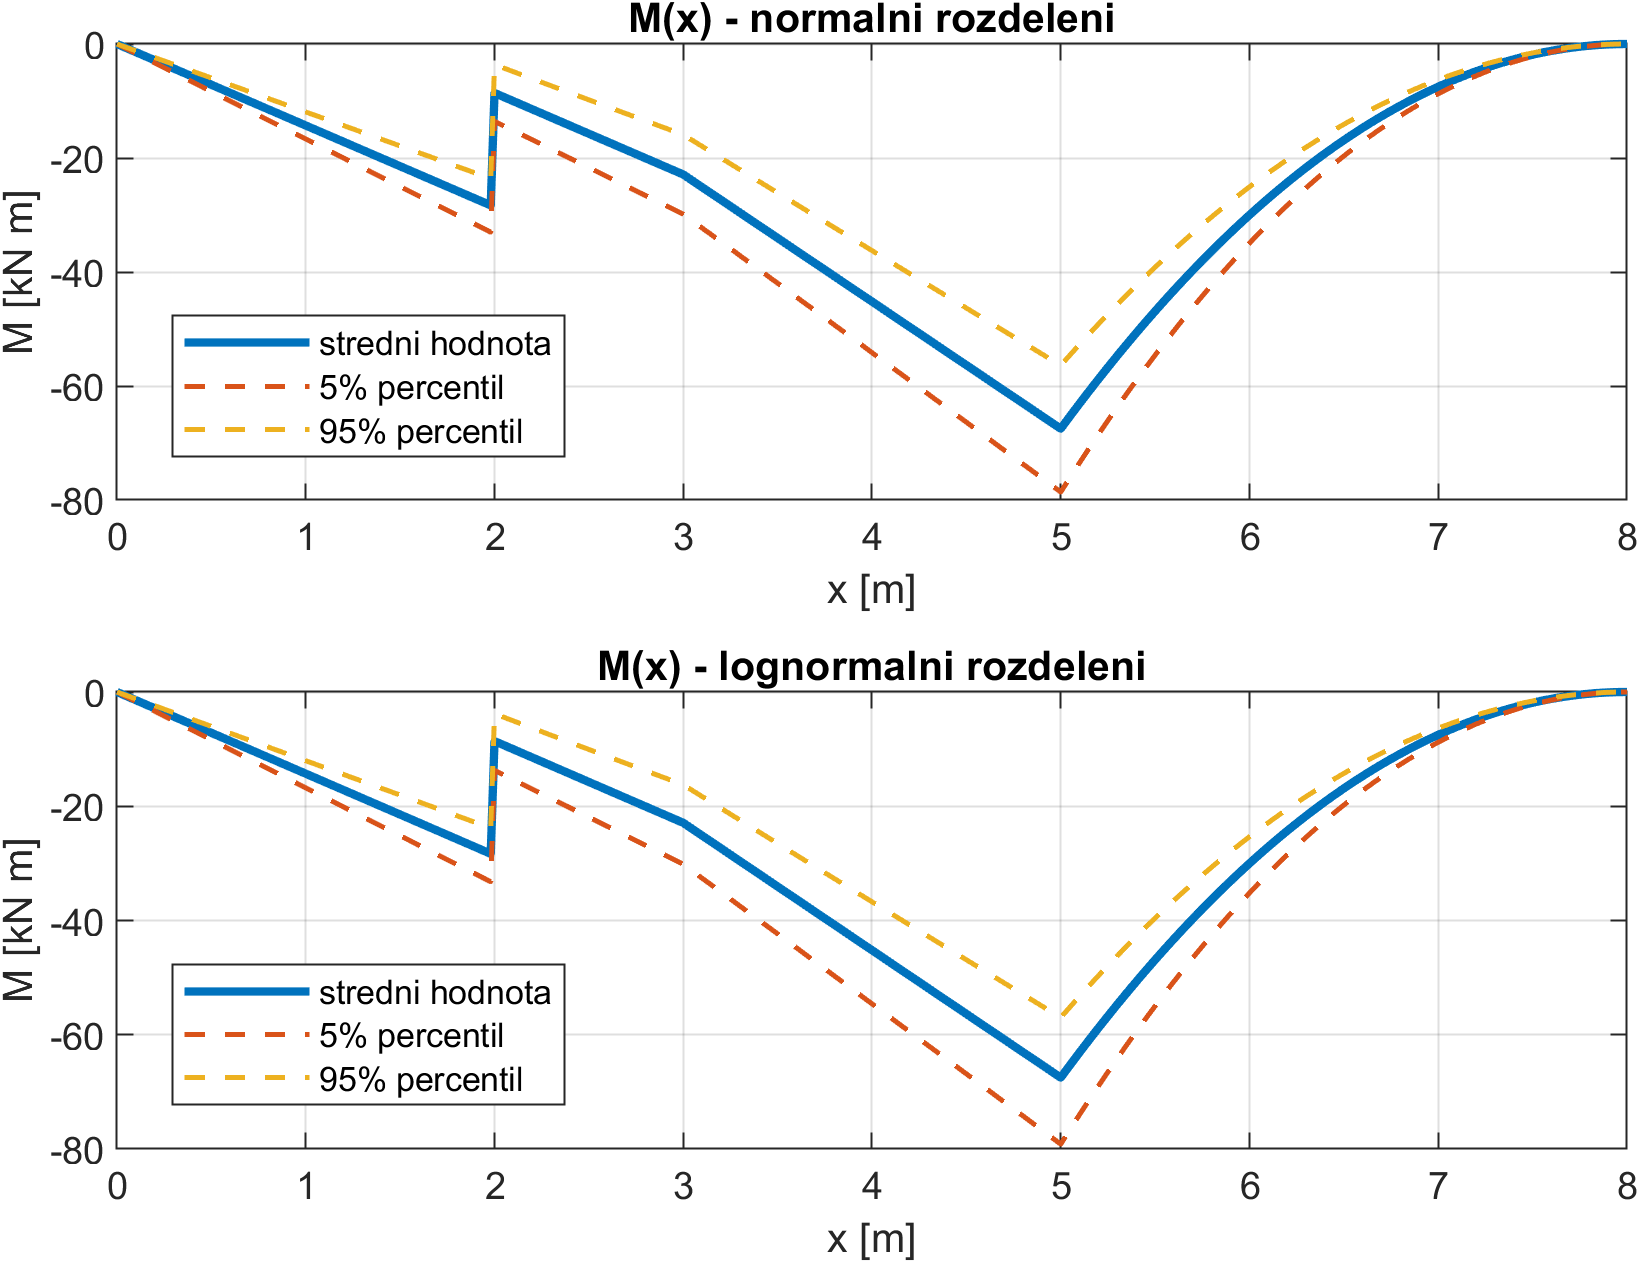
\includegraphics[width=\textwidth,height=0.30\textheight,keepaspectratio]{03_stochasticky_prubeh_M.png}
		{\small (b) Ohybový moment \(M(x)\)}
	\end{minipage}
	
	\caption{Stochastické průběhy posouvající síly \(T(x)\) a ohybového momentu \(M(x)\). Plná čára představuje střední hodnotu, přerušované čáry odpovídají 5\% a 95\% percentilu.}
	\label{fig:stochasticke_prubehy}
\end{figure}

Obr. \ref{fig:stochasticke_prubehy} ukazuje střední průběhy vnitřních účinků a jejich percentilové meze. Šířka percentilového pásma vyjadřuje, jak výrazně se mohou průběhy \(T(x)\) a \(M(x)\) měnit vlivem náhodnosti zatížení. V místech, kde se percentilové křivky sbíhají, je výsledek určen okrajovou podmínkou nebo rovnováhou.

\begin{figure}[H]
	\centering
	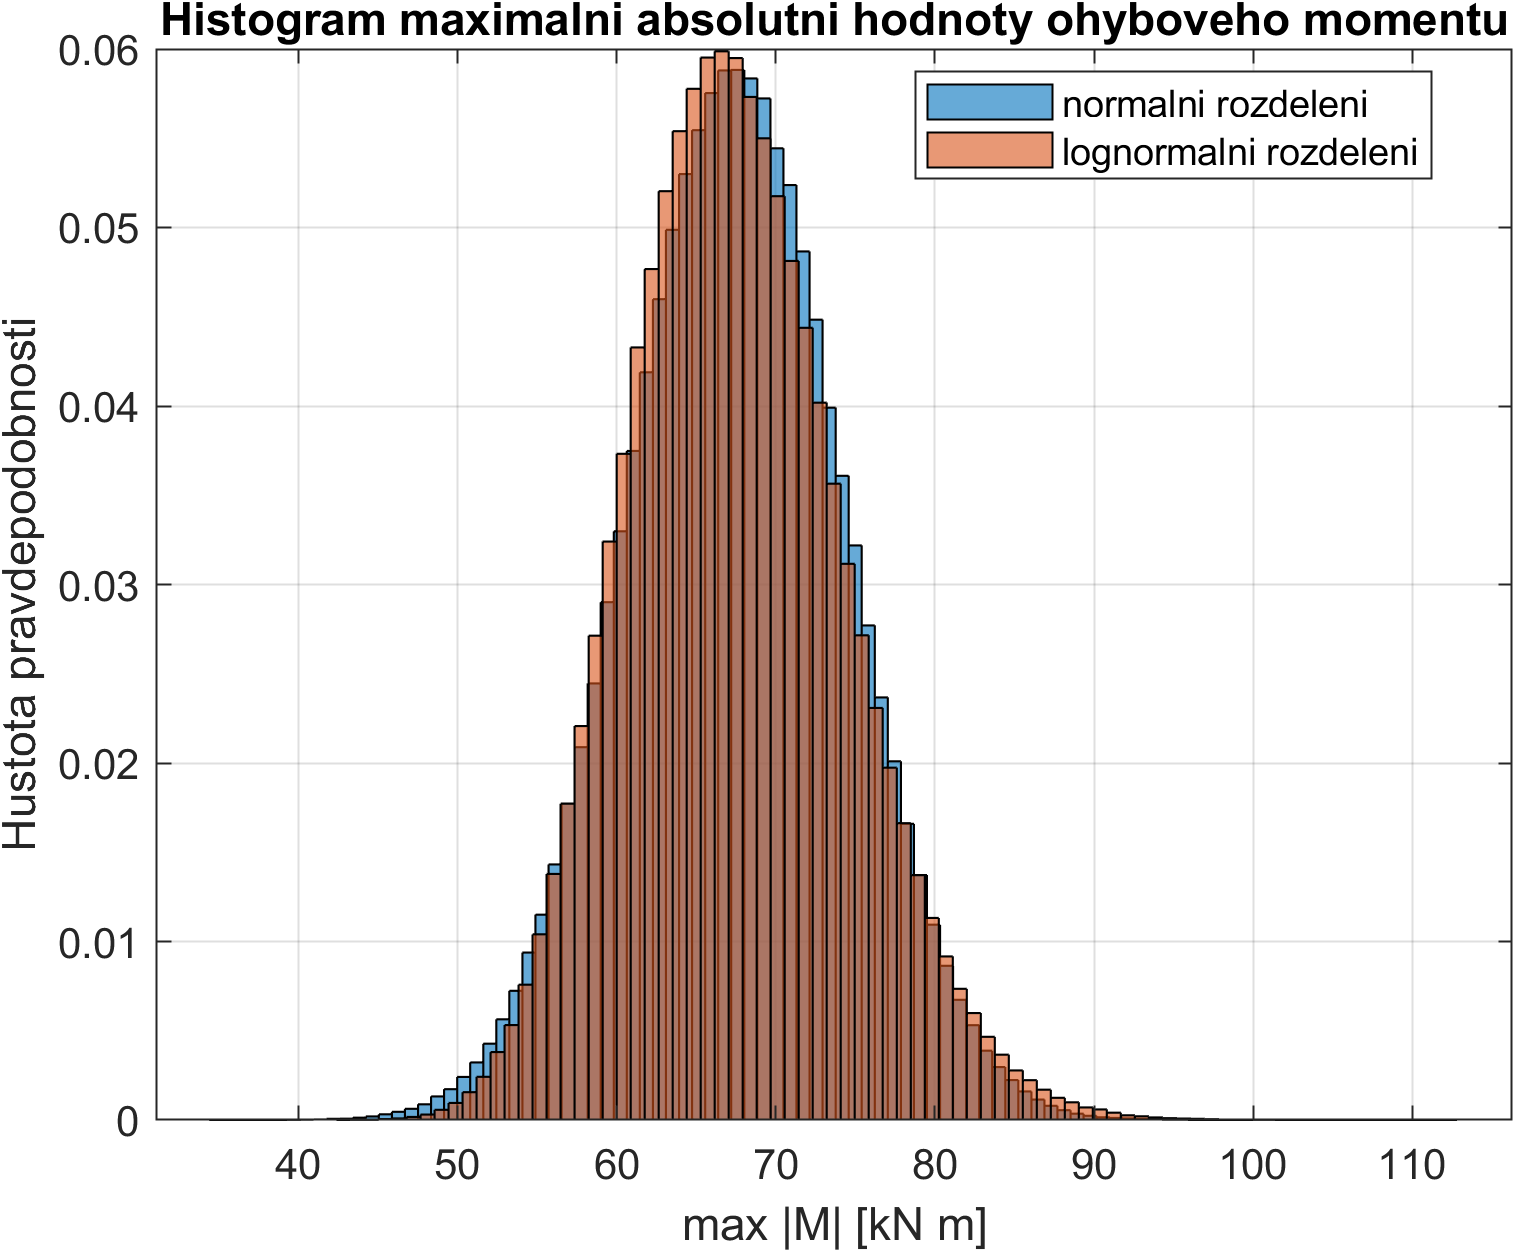
\includegraphics[width=0.92\textwidth,height=0.32\textheight,keepaspectratio]{04_histogram_max_abs_M.png}
	\caption{Histogram maximální absolutní hodnoty ohybového momentu \(\max |M|\) pro normální a lognormální rozdělení zatížení.}
	\label{fig:hist}
\end{figure}

Na obr. \ref{fig:hist} je uveden histogram maximální absolutní hodnoty ohybového momentu. Histogram ukazuje, jak často se v simulacích vyskytovaly jednotlivé hodnoty \(\max |M|\), a doplňuje tak percentilové vyhodnocení o pravděpodobnostní rozdělení maximálního ohybového účinku. Výsledky pro normální a lognormální rozdělení se téměř překrývají. Nejčastější hodnoty se nachází v okolí střední hodnoty přibližně \(67{,}5\,\mathrm{kN\,m}\).

\subsection*{Závěr}

Deterministický výpočet pro střední hodnoty zatížení poskytl reakce \(R_A=-14{,}3\,\mathrm{kN}\), \(R_B=67{,}3\,\mathrm{kN}\) a maximální absolutní ohybový moment \(\max |M|=67{,}5\,\mathrm{kN\,m}\).

Stochastické vyhodnocení metodou Monte Carlo umožnilo kromě středních hodnot určit také rozptyl výsledků. Hodnoty 5\% a 95\% percentilu vymezují oblast, ve které se nachází přibližně 90~\% simulovaných výsledků. Histogram maximálního ohybového momentu dále ukazuje, které hodnoty \(\max |M|\) se v simulacích vyskytovaly nejčastěji.

Výsledky pro normální a lognormální rozdělení byly téměř shodné. V této úloze tedy volba rozdělení neměla zásadní vliv na průběhy vnitřních účinků ani na maximální ohybový moment. Hlavním důvodem je nízký variační koeficient \(v=0{,}1\), při kterém se obě rozdělení výrazně neliší.

\end{document}
